\makeatletter
\def\input@path{{../}}
\makeatother

\documentclass[/main.tex]{subfiles}

\begin{document}
\graphicspath{{./pics/}{ch3/pics/}}

\textpages
\chapter{Simulating the \MJD}

\section{Introduction}


\section{Simulation Software}
\subsection{\Mage}
\Mage\ (Majorana/Gerda) \cite{mage2011} is a Monte Carlo software package developed jointly by the \MJ\ and \Gerda\ collaborations for the purpose of simulating low-background experiments involving HPGe detectors.
\Mage is written primarily in \cpp\ and is based on the \geant\ physics simulation framework\cite{geant2003}.
A \geant\ simulation requires the following inputs:
\begin{itemize}
\item{\textbf{Experiment Geometry:}}
  A discription of the physical dimensions, location, and materials must be provided.
  These should be included for both the detectors and the experimental structure surrounding the detectors.
\item{\textbf{Event Generator:}}
  A generator creates the initial conditions for an event, including the initial particles generated, and the intitial positions and momenta of each initial particle.
  The initial positions will typically be sampled from a particular subset of the full experimental geometry, such as the volume defined by a particular component.
  The initial momenta will be sampled from the allowed phase space of the process, conserving energy and momentum and sampling the angular correlation distribution.
  Many processes will generate multiple events; for example, a \Th{228} decay will generate a set of particles for each decay in the chain, including $\gamma$s generated by nuclear deexcitations.
\item{\textbf{Physics Lists:}}
  The physics lists describe the physical processes to be simulated as the generated particles propagate through the experimental geometry.
  Examples of such processes include Compton scattering of $\gamma$-rays in matter and energy deposition of electrons as they propagate through matter.
  A physics list will describe the probability of a process happening in a given material, any changes to the particle that generated the process, and any new particles produced by the process.
\end{itemize}
\Mage\ contains geometries describing various detector configurations for the \MJD.
\Mage\ also includes event generators that are used to describe \bb from inside the detectors, backgrounds generated by various experimental components from various isotopes, and the line sources used in detector calibration.
Finally, \Mage\ includes the relevant physics lists to the nuclear processes observed by the \MJD.
\Mage\ enables a user to select a geometry and event generator by writing a simple macro and running the \texttt{MaGe} executable on that macro.
All simulations described in this chapter will use the full as-built \MJD\ geometry, which is shown in figure~\ref{fig:mageasbuilt}.
\\
\begin{figure}[h]
  \centering
  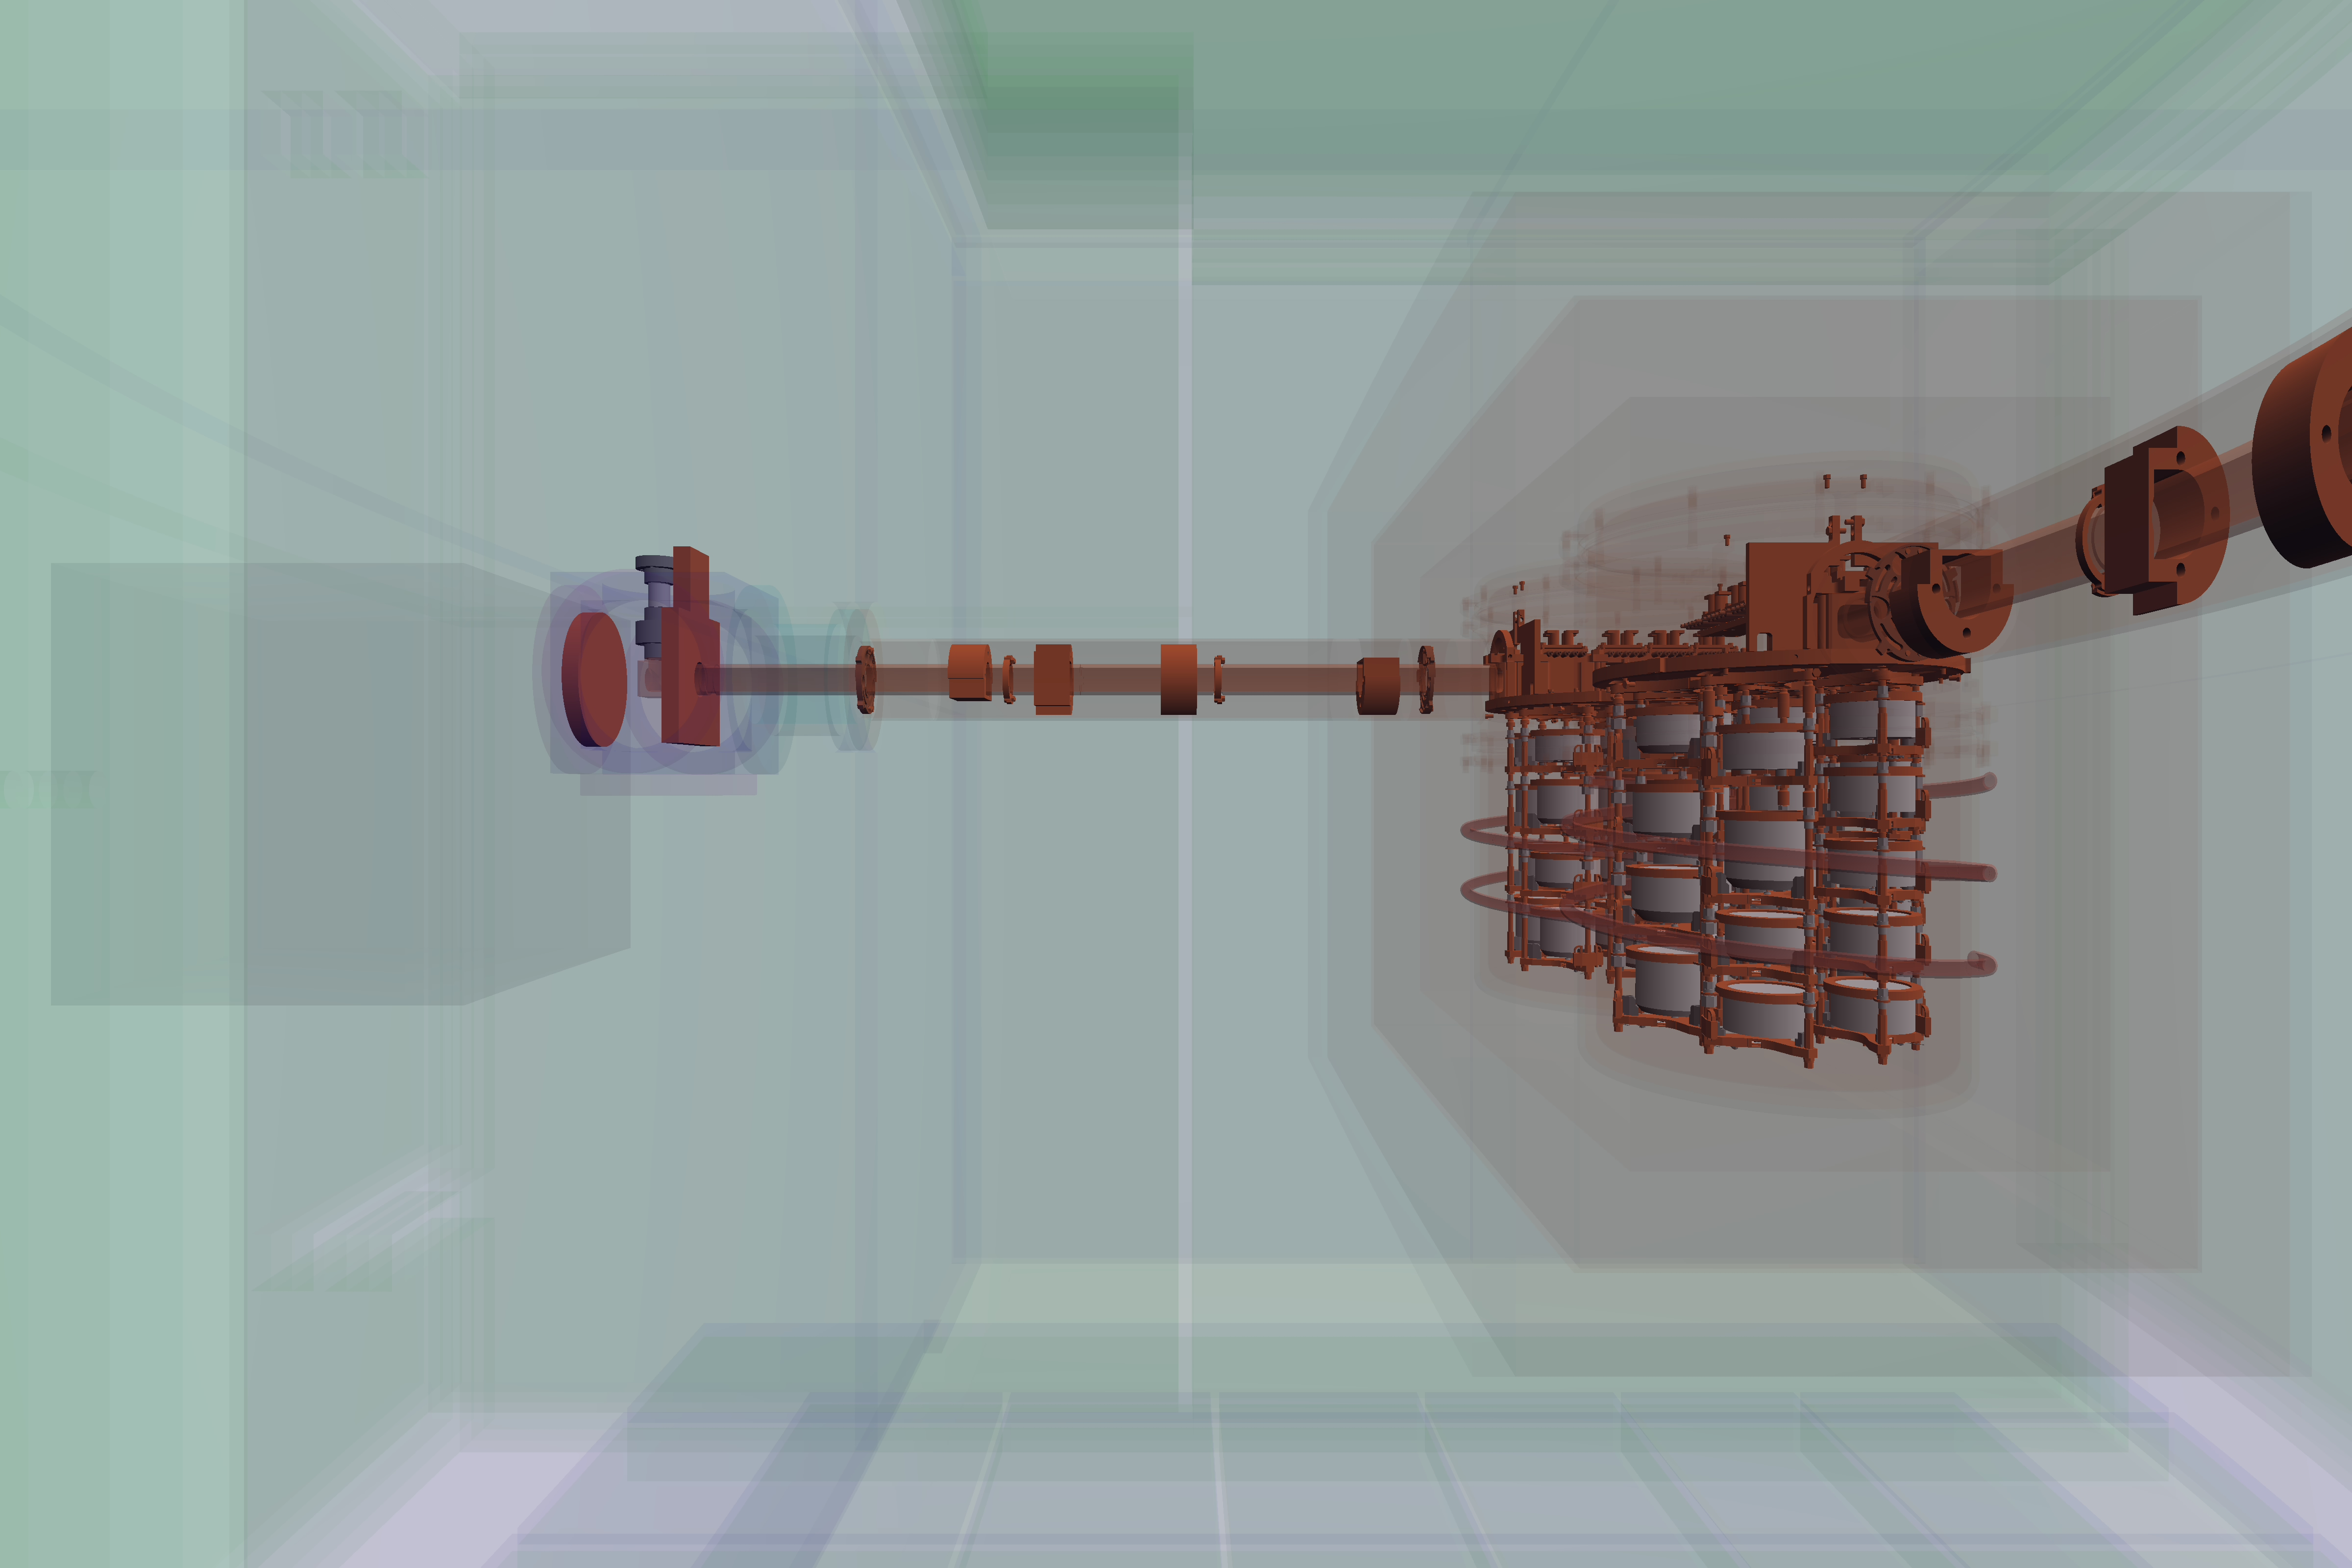
\includegraphics[width=0.8\textwidth]{Geant4Geom.jpeg}
  \caption[The \MJD\ as built simulated geometry]{\label{fig:mageasbuilt}
    The as-built \MJD\ geometry as programmed in \Mage.
  }
\end{figure}

A Monte Carlo run by \geant\ will generate a large number of event primaries.
A Monte Carlo event primary begins with the set of particles created by the input event generator.
Each particle will then be given a particle track, describing the path it takes through the experiment geometry.
If the particle undergoes an interaction with the experiment as described in a physics list, the particle track will end and a Monte Carlo step will occur.
A Monte Carlo step describes the particle before and after an interaction, any additional particles generated in the interaction, and the amount of energy imparted into the matter at the site of the interaction.
For each Monte Carlo event primary, \Mage\ will record an event with the details of each Monte Carlo step that occurs inside of a detector, including the position of the step, the incoming particle, the outgoing particles, the physics process that caused the step, and the amount of energy deposited.
If no interactions occur inside of a detector, no event will not be recorded, but recorded events are enumerated according to the event primaries to ensure that the detection efficiency can be accurately counted.
\\
The simulation events are stored in a \TTree\ containing the following branches:
\begin{itemize}
\item{\texttt{fMCRun}:}
  Contains meta-information about the simulation run, including the run number, number of events, and settings for the run.
\item{\texttt{eventHeader}:}
  Contains meta-information about the event such as the event ID.
\item{\texttt{eventSteps}:}
  Contains data from each event step that deposits energy in a HPGe detector volume, including the location, process and energy deposition.
\item{\texttt{eventPrimaries}:}
  Contains data from the first step in an event, which generated the event.
\end{itemize}

\subsection{Simulation Post-Processing} \label{sec:simpostproc}
Once a \Mage\ simulation is run, the data generated must be post-processed to look like \MJD\ data.
Post-processing is performed by the GAT executable \texttt{process\_MJD\_as\_built\_mage\_results}.
The post-processor requires the input of individual detector characteristics such as energy resolution and dead layer parameters, which are provided via a JSON file.
The relevant steps of the posts-processor will be described in the next few paragraphs.
\\
First, steps within 0.1~mm and 5~ns of each other are grouped into clusters.
A typical cluster will contain the initial physics process that generated the cluster, such as a Compton scatter or $\beta$ decay which generate a high energy electron in the detector, and many electron scatters as the electron comes to rest inside of the detector, generating a cloud of electron-hole pairs.
For each cluster, the total energy and energy-weighted average position of the cluster are computed.
\\
The effect of the detector dead layers are computed for each step individually.
The fraction of total charge collected is modelled as a function of depth beneath the detector surface by the piecewise function
\begin{equation}
  A(x) = \begin{cases}
    0 & z < 0 \\
    g(x)=Ae^{Bx} + C & 0 \leq z < t \\
    h(x)=Mx + D & t \leq z < 1 \\
    1 & t \geq 1
  \end{cases}  \qquad
  \text{Constrained to: } \begin{cases}
    g(0)\equiv 0 \\ g(t)\equiv h(t)\equiv f \\ g'(t)\equiv h'(t) \\ h(1)\equiv 1
  \end{cases}
\end{equation}
where $x$ is the depth of the event as a fraction of the dead layer thickness, $t$ is the transition depth, $f$ is the transition fraction, and all other parameters are uniquely determined by $t$ and $f$ \cite{giovenetti2015phd}\cite{buuck2018}.
For each cluster, the uncollected charge is summed and used to compute the deadness fraction for the cluster.
The total measured energy is computed by summing the energy of each cluster, degraded by a factor of its deadness, in a single detector.
The deadness model parameters are measured by performing a fit of a simulated \Th{228} calibration spectrum to calibration data, floating the dead layer parameters for each detector.
The most sensitive parts of the calibration spectrum in this fit are the low energy portion of the spectrum, where events occur in the transition layer and have degraded energy, and in peak heights.
The parameters for this model are provided individually for each detector in a JSON file input to \texttt{process\_MJD\_as\_built\_mage\_results}.
\\
Finally, the post-processor smears energies by the response function measured during \Th{228}\ calibration runs.
The post-processor uses the peakshape functions described in appendix~\ref{appendix:peakfitter}.
Only the gaussian and low energy tail parameters are used.
The post-processor samples an energy from the probability distribution described by the peak-shape function centered at the energy calculated for the event.
The peak-shape parameters are provided individually for each detector using the input JSON file.

\subsection{Simulation Skimming} \label{sec:simskim}
Finally, skim files are produced containing parameters of interest from the post-processed files using the software \texttt{es\_skimsims}.
Skim files also mix postprocessed files from multiple sources in ratios corresponding to the various activities of the sources.
\texttt{es\_skimsims} accepts as input a json file listing the simulated sources, the desired activity of each source, and the number of available event primaries.
From this, it calculates the number of primaries to accept from each source by maximizing the total number of events used while mainting the correct ratio according to the activities.
Once this is done, it goes through each source sequentially and saves parameters of interest, including energy and detector position to a \texttt{TTree}.
As will be discussed in future chapters, single detector events are of little interest to this analysis, so only \msmd\ events are recorded in order to maintain a small file size.
Multiplicity 1 events are recorded separately to a histogram according only to energy.
The skimming process also accounts for which sets of detectors are enabled.
Another input of \texttt{es\_skimsims} is a json file containing a list of detector configurations, containing a bitmask describing which detectors are and are not enabled.
The detector configurations will be discussed further in section~\ref{sec:sds}.
When the skimmer encounters a disabled detector in an event, it ignores that detector, and does not count it towards the event multiplicity.
\\
 
Each detector spends some portion of operating time dead, due to the finite rate at which the digitizers can retrigger, which can cause up to $\sim1$\% of HPGe hits to fail to read.
This effect is assumed to be random and uncorrelated between detectors.
The dead time of each detector is measured by counting the number of pulser events in each detector for each run.
Because the pulses occur at a fixed rate, we can predict the number of pulser events that should occur in any given run; the fraction of pulser events missed is assumed to represent the dead time.
The json detector configuration file contains the dead time fraction and the statistical uncertainty on that fraction for each active detector.
For each simulated detector hit, the data skimmer randomly throws out hits according to the the probability represented by the dead fraction, treating that detector as inactive for that event.

\section{Simulation of Excited State Decays}

\begin{figure}
  \centering
  \includegraphics[width=.9\linewidth]{ESsim}
  \caption[Simulation of multiplicty 2 events from \tnbb\ to \SP{0}{+}{1}]{
    Multiplicity 2 energy spectrum produced by a decay0 simulation of \tnbb\ of \Ge{76} to the \SP{0}{+}{1} state of \Se{76}.
  }
\end{figure}

\section{Background Model Simulation}

\begin{figure}
  \centering
  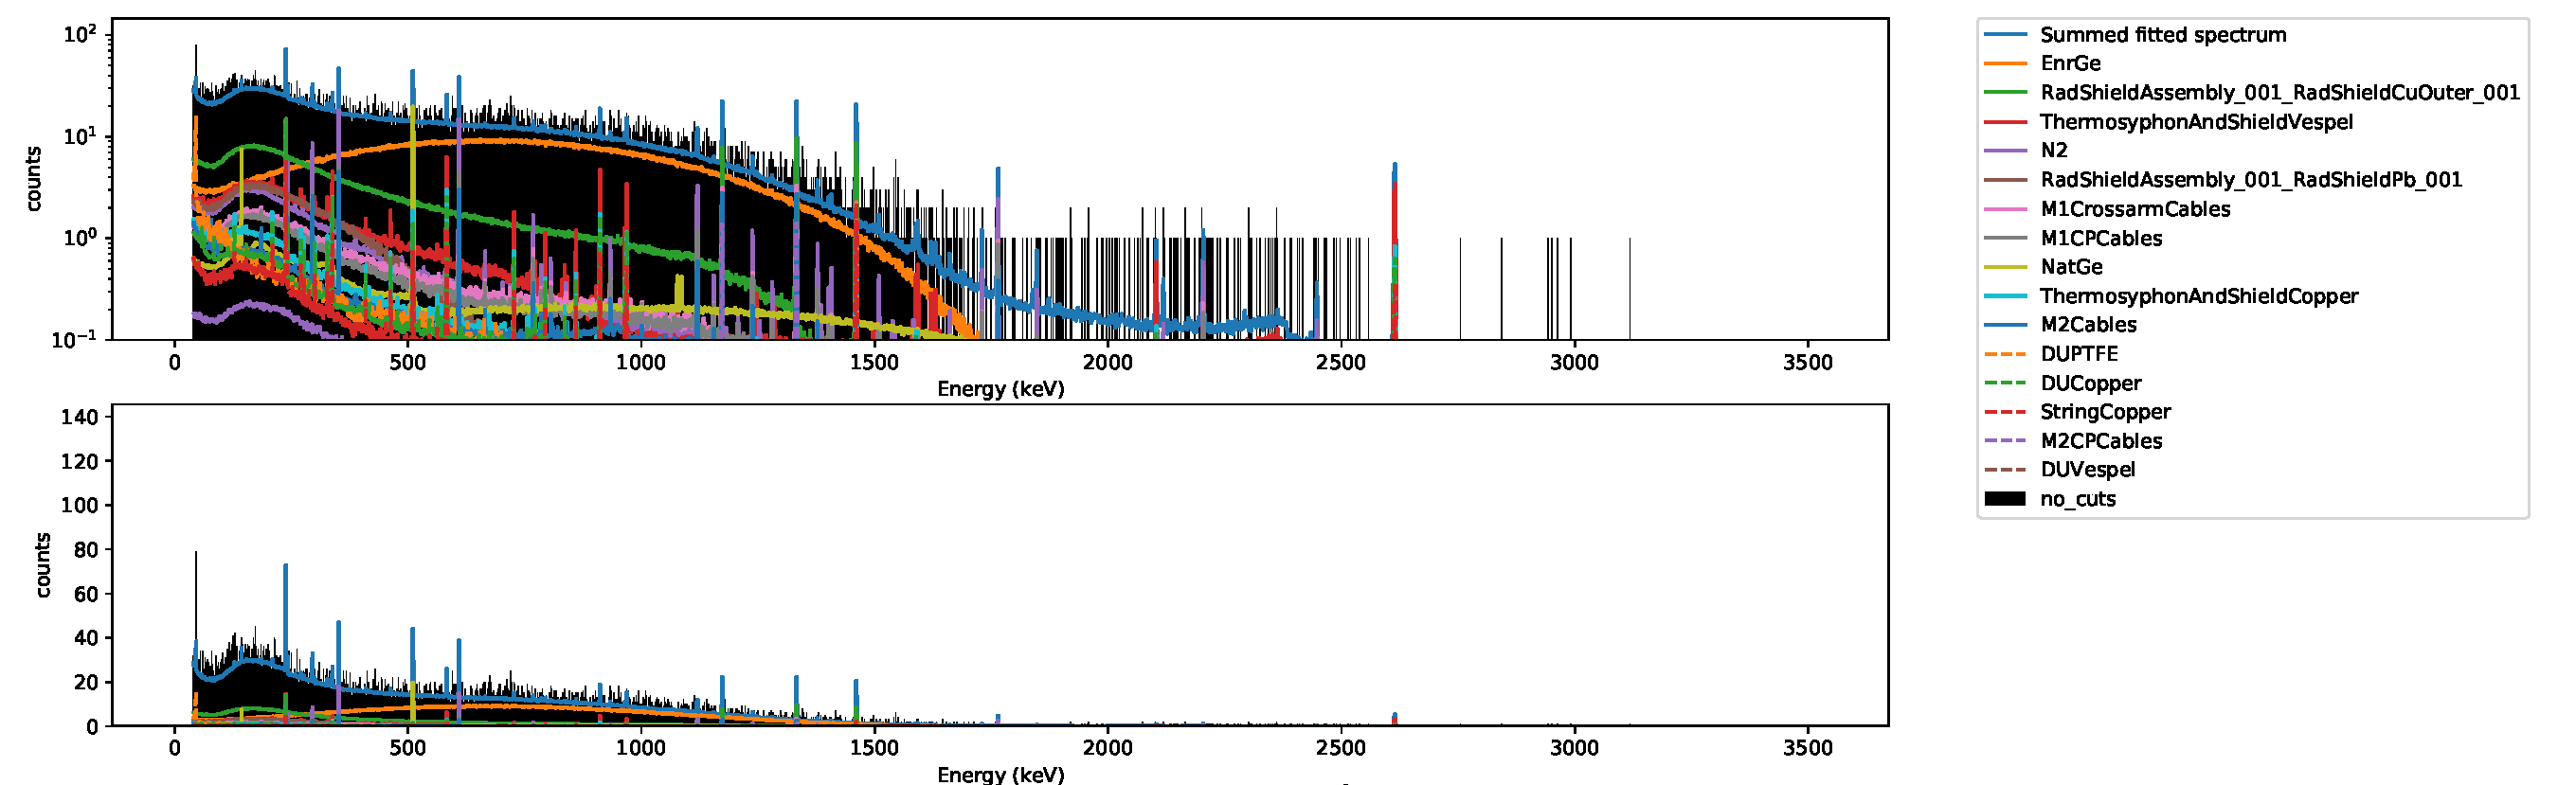
\includegraphics[width=1\linewidth]{BGsim1D}
  \caption[Simulation of multiplicty 1 events from the background model]{
    Energy spectrum of multiplicity 1 events produced from a simulation of the background model, with most common source components labelled.
  }
\end{figure}

\begin{figure}
  \centering
  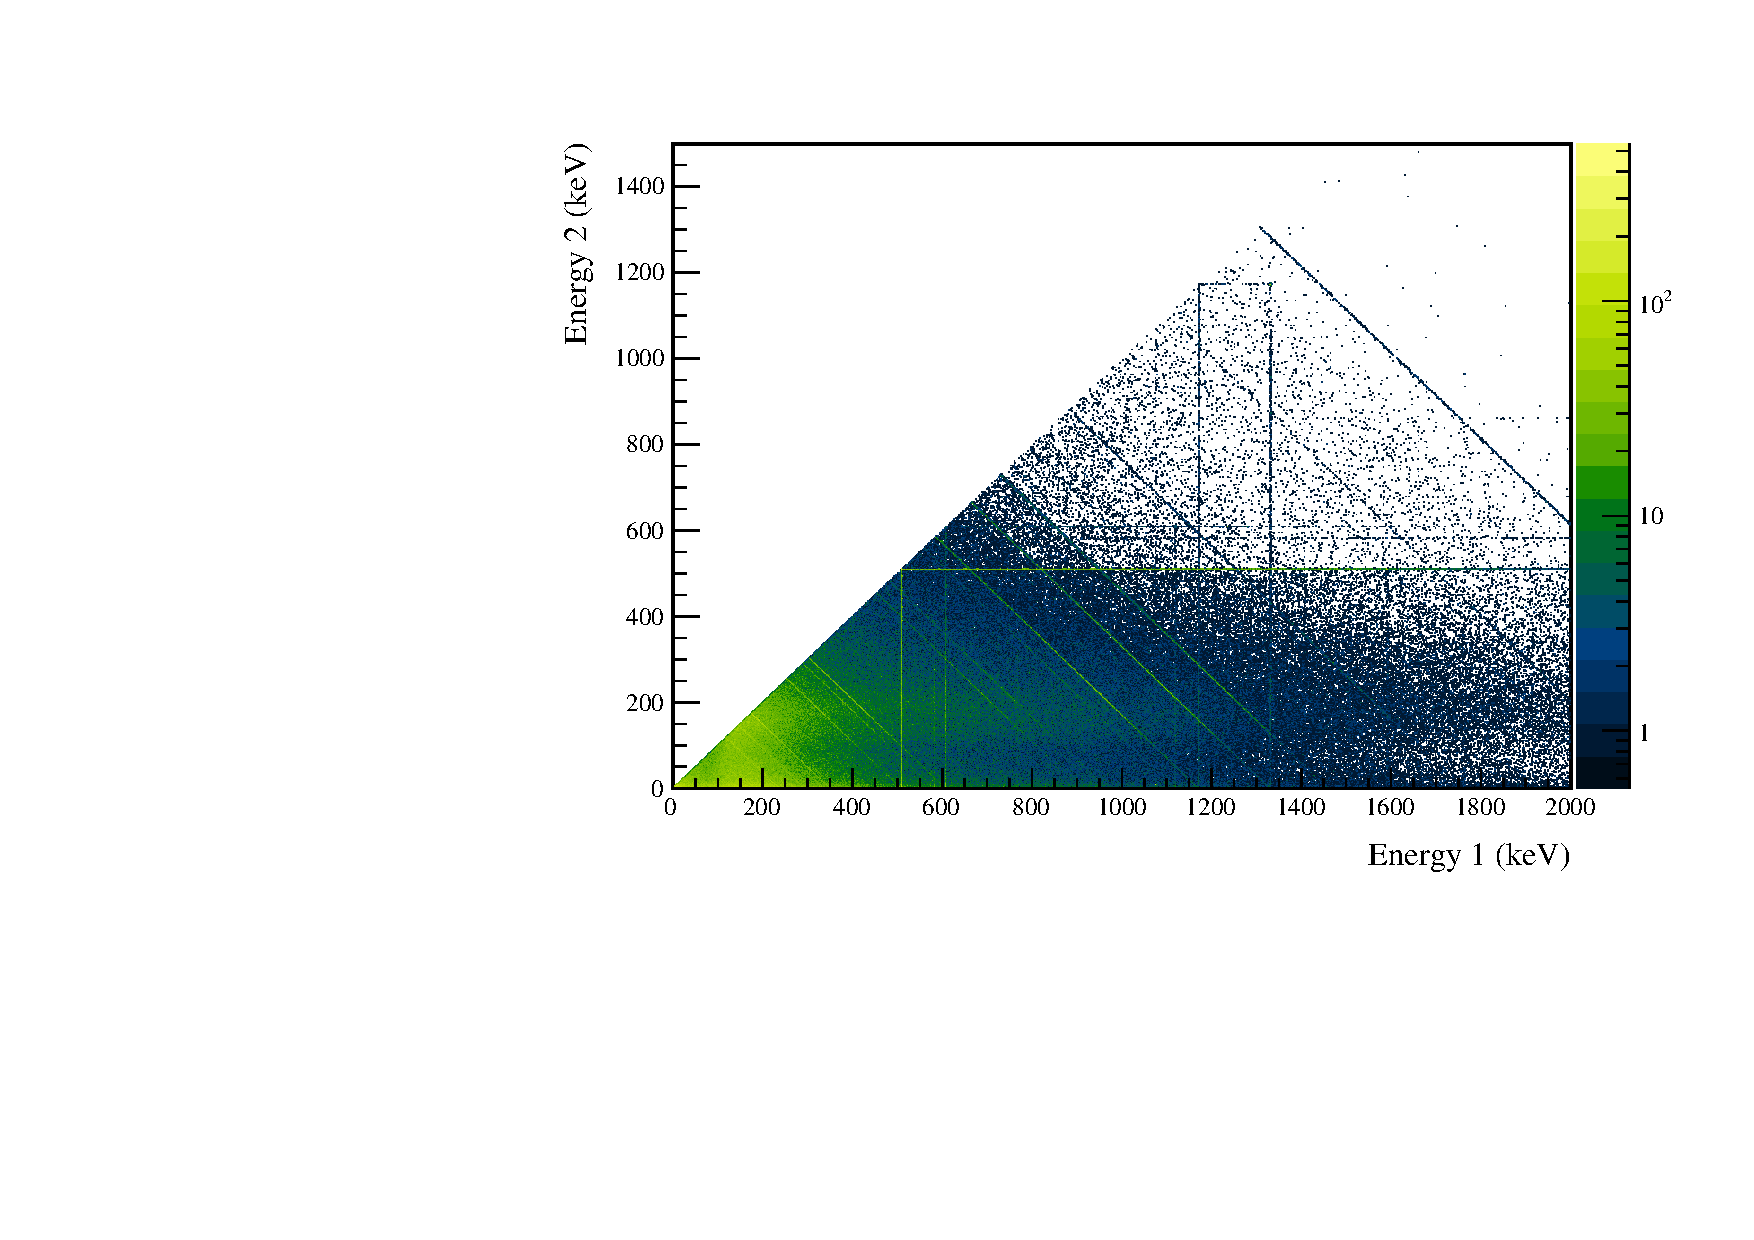
\includegraphics[width=.9\linewidth]{BGsim2D}
  \caption[Simulation of multiplicty 2 events from the background model]{
    Multiplicity 2 energy spectrum produced by a simulation of a preliminary version of the \MJD\ background model.
  }
\end{figure}

\section{Calibration Source Simulation}

\begin{figure}
  \centering
  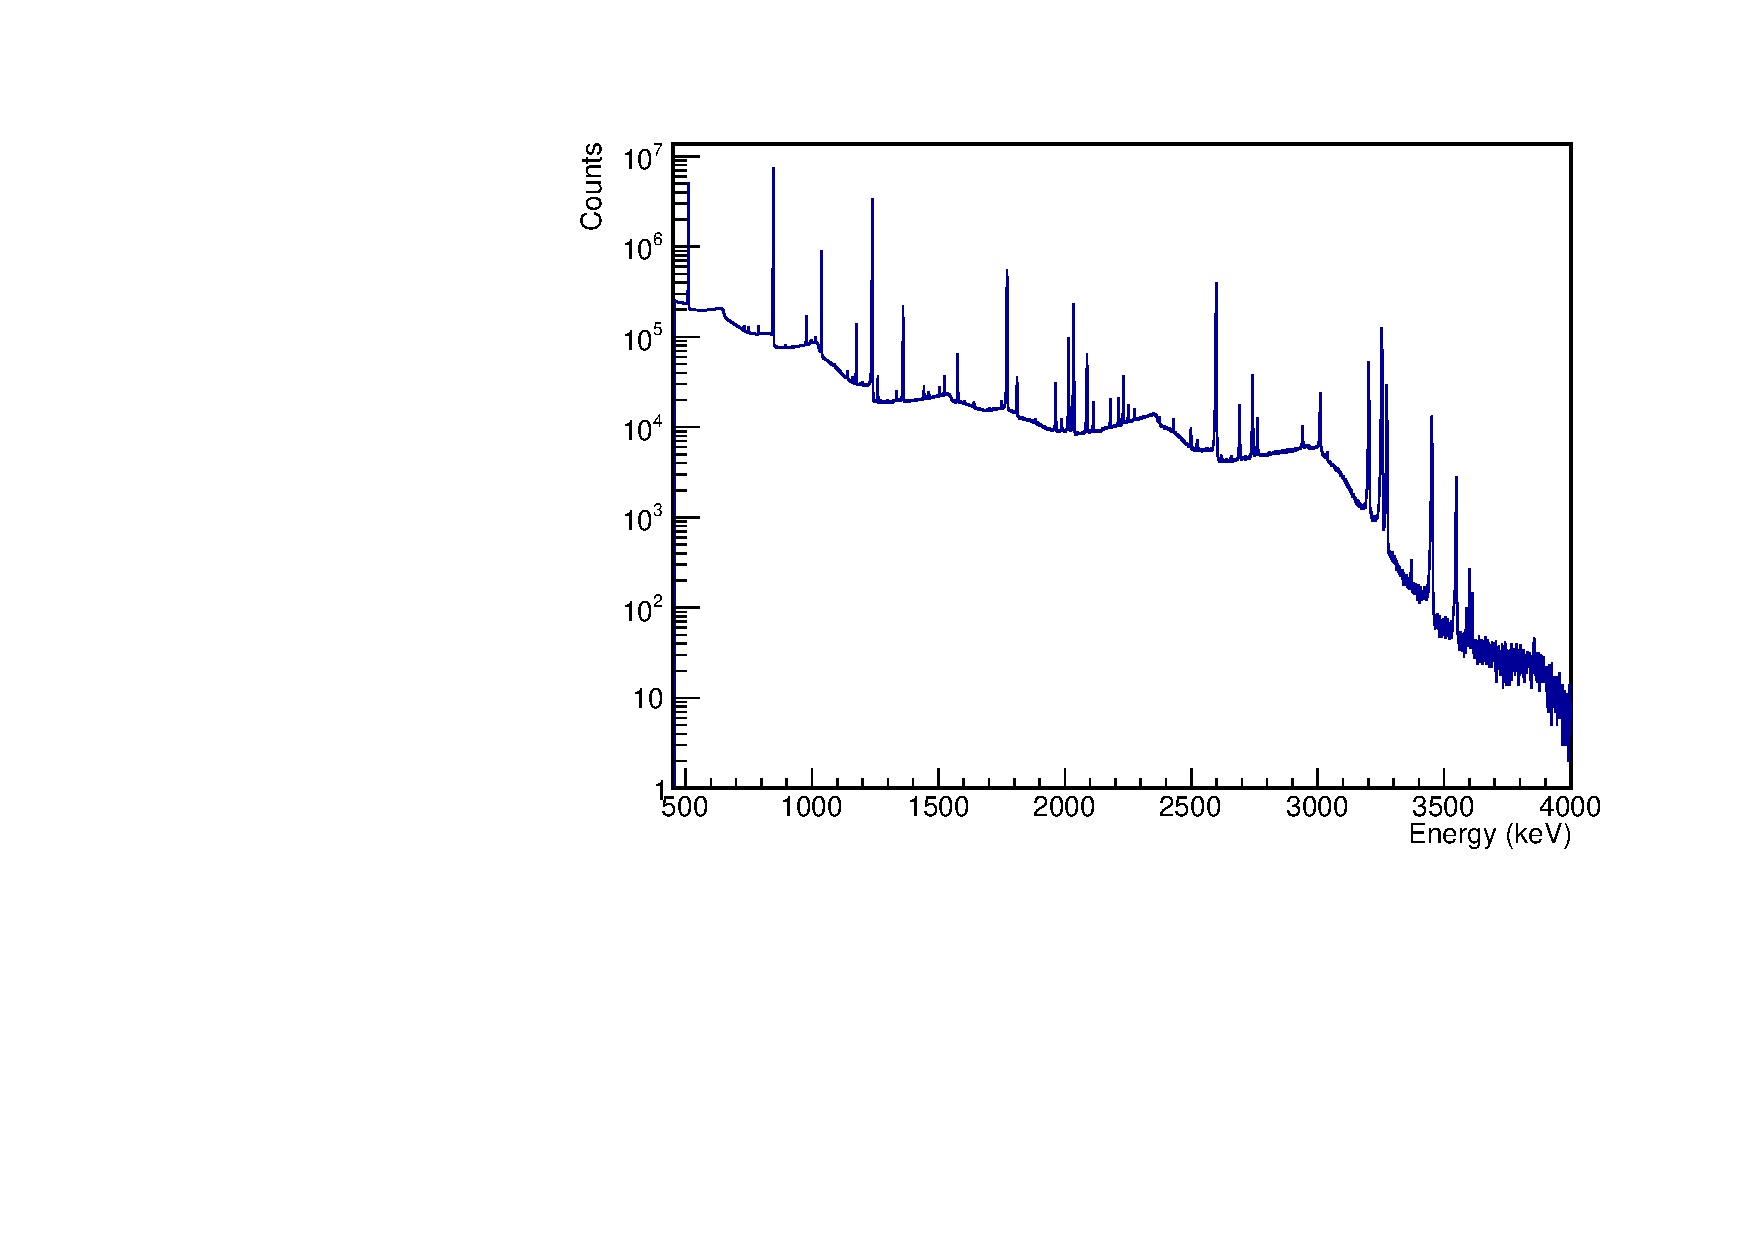
\includegraphics[width=.8\linewidth]{Co56Sim1D}
  \caption[Simulation of multiplicty 1 events from \Co{56} line source]{
    Energy spectrum of multiplicity 1 events produced from a simulation of the \Co{56} line source inserted into the module~1 calibration track.
  }
\end{figure}

\begin{figure}
  \centering
  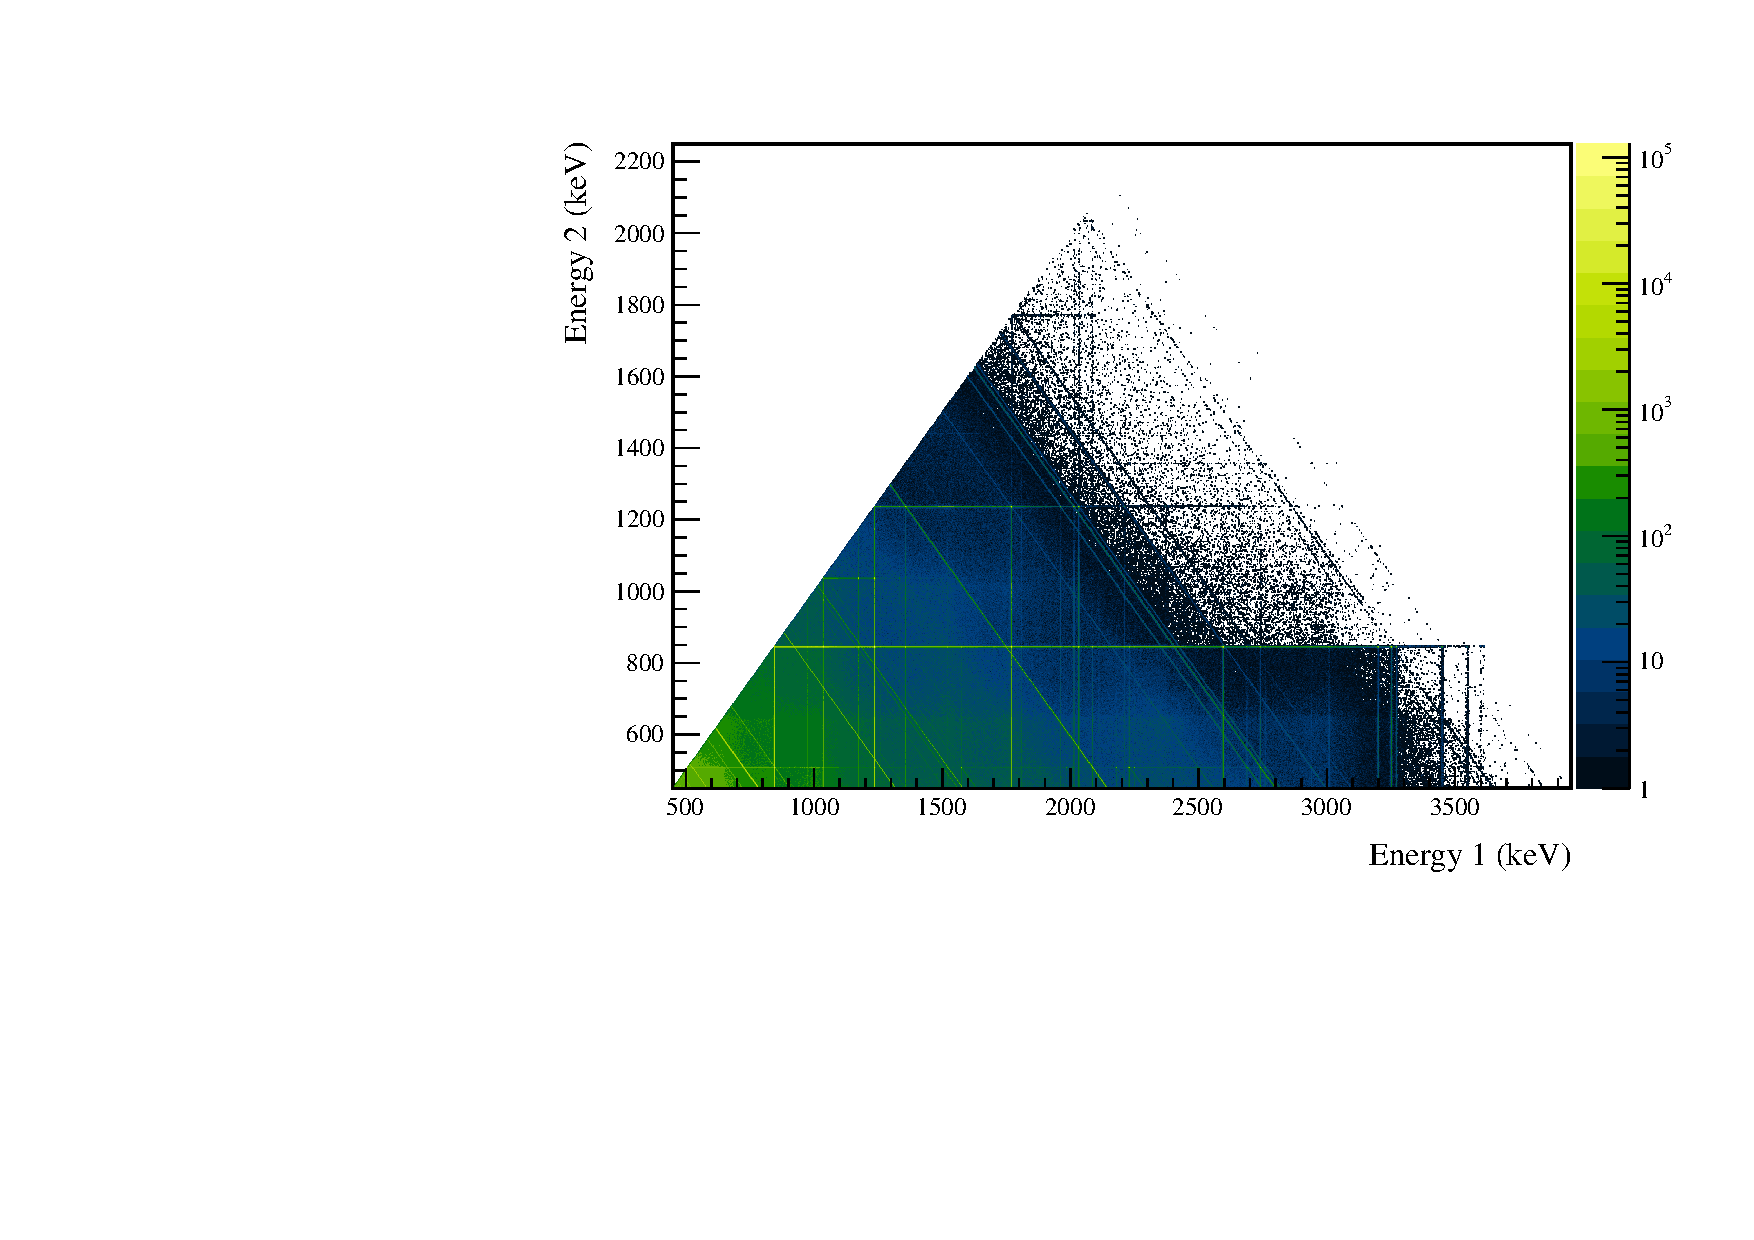
\includegraphics[width=.8\linewidth]{Co56Sim2D}
  \caption[Simulation of multiplicty 2 events from \Co{56} line source]{
    Multiplicity 2 energy spectrum produced by a simulation of the \Co{56} line source inserted into the module~1 calibration track.
  }
\end{figure}


\end{document}
